\chapter{Resultados}

El problema de llevar inventario de un a\~no a otro se resolvi\'o f\'acilmente con el m\'etodo \textit{Q-learning}, pues su misma estructura requiere valores descontados de los estados futuros en cada estado presente. Para lograr el mismo efecto con el m\'etodo \textit{Policy Iteration}, ser\'ia necesario crear artificialmente d\'ias de entrenamiento antes y despu\'es del periodo de 365 d\'ias en el que los agentes est\'an aprendiendo, sin embargo, esto a\~nadir\'ia complejidad computacional.

\section{El Mundo y los Agentes}

A pesar de que nuestro sistema tiene seis roles, en realidad solamente cuatro de ellos toman decisiones:

\begin{itemize}
    \item El consumidor \textbf{obedece} a su necesidad interna de cerveza, mayor en fines de semana y festividades
    \item La tienda minorista \textbf{decide} cu\'anta cerveza va a comprar a la tienda de mayoreo
    \item La tienda de mayoreo \textbf{decide} cu\'anta cerveza va a comprar al almac\'en regional
    \item El almac\'en regional \textbf{decide} cu\'anta cerveza va a comprar a la f\'abrica
    \item La f\'abrica \textbf{decide} cu\'anta cerveza va a comprar a los campos
    \item Los campos \textbf{obedecen} a sus ciclos de siembra y cosecha
\end{itemize}

A pesar de que, estrictamente, en nuestro sistema multiagente todos los roles son agentes, por claridad en la descripci\'on y el flujo del c\'odigo nos referiremos como agentes solamente a aquellos roles que toman decisiones. Las ecuaciones de los agentes en los extremos ``encajan'' si suponemos que, para el consumidor, su \textit{policy} \'optimo es su demanda normal durante el a\~no, y para los campos, es su producci\'on.

Durante el aprendizaje, todos los agentes siguen el mismo conjunto de reglas (aprender cu\'anto tienen que comprarle al agente superior en cada d\'ia), as\'i que las ecuaciones de ganancia y aprendizaje son las mismas. En este trabajo, usaremos la siguiente construcci\'on del mundo, con cierta notaci\'on para los distintos par\'ametros del mundo:

\begin{enumerate}
    \item Para cada agente \textit{$a$}, el agente superior en la cadena de suministro es \textit{$a+1$}; el inferior es \textit{$a-1$}
    \item Cada agente tiene un precio de venta \textit{$p_{a}$}, un costo de almacenamiento \textit{$c_{a}$} y un costo por orden no cumplida (\textit{backlog}) \textit{$b_{a}$}
    \item En cada d\'ia \textit{$d$}, cada agente \textit{$a$} recibir\'a del agente superior \textit{$a+1$} la cantidad demandada por el primero en el d\'ia \textit{$d-1$}, sujeto a que tal cantidad sea menor o igual a la cantidad que el agente \textit{$a+1$} ten\'ia en el almac\'en
    \item En cada una de estas transacciones, cada agente recibe el dinero equivalente, basado en su respectivo precio de venta, e incurre en costos de almacn\'en y por \'ordenes no cumplidas
\end{enumerate}


Esto quiere decir que, independientemente del algoritmo de aprendizaje que usemos, cada agente \textit{a} calcula su ganancia en el d\'ia \textit{d} de la siguiente manera:

$$
ganancia_{a,d} = (p_{a} * ventas_{a, d}) 
$$
$$
\quad  \quad  \quad  \quad  \quad  \quad  \quad  \quad  \quad \quad  \quad   \quad  \quad - (b_{a}* (demanda_{a-1,d} - ventas_{a,d})) 
$$
$$
\quad  \quad  \quad  \quad  \quad  \quad  \quad  \quad - (p_{a+1}*ventas_{a+1, d-1})
$$
$$
\quad  \quad  \quad  \quad  \quad  \quad  \quad  \quad - (c_{a}*inventario_{a,d-1})
$$

Es decir, cada agente recibe el dinero correspondiente a las ventas que hace al agente inferior, paga el costo castigo relacionado a las \'ordenes no cumplidas, paga las \'ordenes hechas al agente superior y paga el costo de almacenamiento.\\

Una vez establecidas todas las relaciones entre todos los jugadores y establecidos los par\'ametros del mundo, hemos obtenido dos formas diferentes de solucionar el juego: la primera con \textit{policy iteration} y la segunda con \textit{Q-learning}.

\section{Policy Iteration}

Las ecuaciones que describen el aprendizaje de un agente son:

\begin{enumerate}
    \item La ecuaci\'on de utilidad (reward) para cada agente $a$ en el d\'ia $d$:

$$
R(a, d) = R(a,d) + \gamma*r_{a, d+1} + ... + \gamma^{364}*r_{a,d+364}
$$

    \item BLA
\end{enumerate}




Bajo este algoritmo, los agentes aprenden \textit{policies} que siguen el comportamiento de la oferta, lo cual es el comportamiento esperado dado que en las especificaciones iniciales, se defini\'o manualmente que el la demanda anual no sobrepasara la oferta anual. Este resultado puede observarse en la figura \ref{politer_policies}. \\

\begin{figure}[ht]
\caption{Policies \'optimas de cada agente bajo \textit{policy iteration}}
\label{politer_policies}
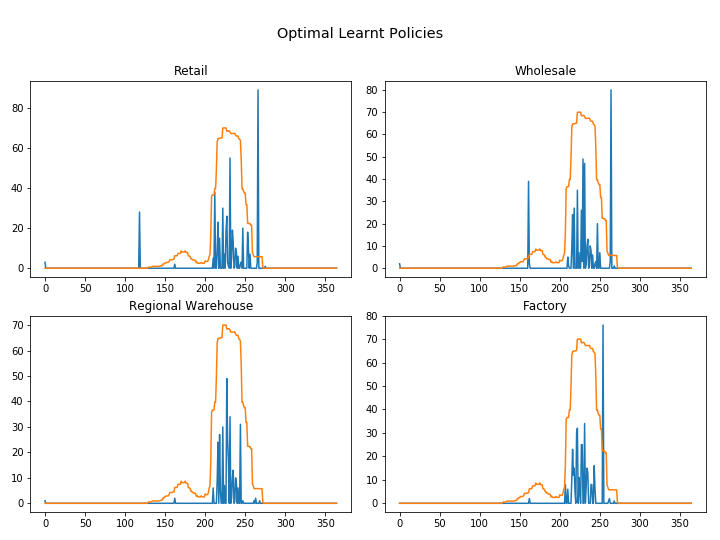
\includegraphics[width=15cm]{tesis_tex/figs/policyiteration_policies.png}
\centering
\end{figure}

Podemos observar que todos los agentes presentan una tendencia positiva al encontrar mejores \textit{policies} en cada iteraci\'on del algoritmo.

\begin{figure}[ht]
\caption{Pagos \'optimos de cada agente}
\label{politer_payouts}
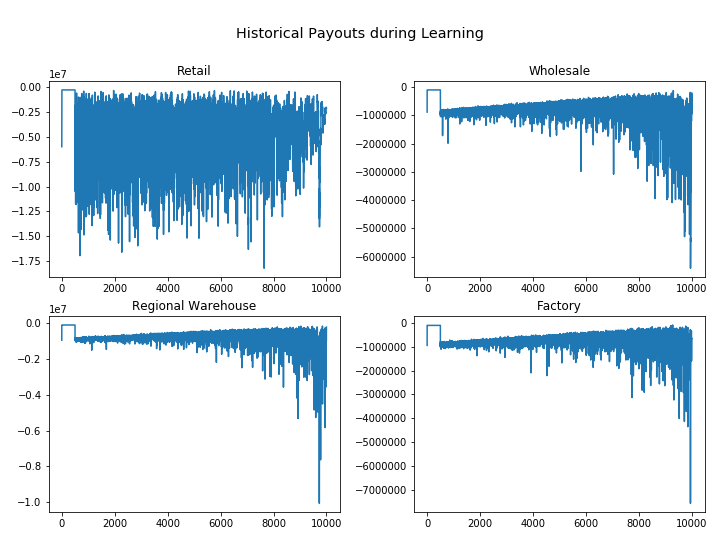
\includegraphics[width=15cm]{tesis_tex/figs/policyiteration_payouts.png}
\centering
\end{figure}

\section{Q-Learning}

A diferencia de \textit{policy iteration}, este m\'etodo encuentra, para cada estado, la acci\'on que acercar\'a al agente lo m\'as posible a la meta. Por supuesto, la \textit{policy} \'optima es equivalente con cualquiera de ambos m\'etodos, pero \textit{Q-learning} nos permite m\'as libertad respecto a empezar a jugar el juego a mitad de a\~no, arreglar malas decisiones tomadas por los agentes en periodos anteriores gracias a su adaptabilidad ante cambios estoc'asticos, etc.\\

Las ecuaciones que describen el aprendizaje de un agente son:

\begin{enumerate}
    \item La ecuaci\'on de utilidad (o recompensa) para cada agente $a$ en el d\'ia $d$:

$$
R(a, d) = r(a,d) + \gamma*r_{a, d+1} + ... + \gamma^{364}*r_{a,d+364}
$$

Donde la recompensa del agente \textit{a} en el d\'ia \textit{d} es la ganancia relacionada a sus respectivas transacciones, como se defini\'o al principio de este cap\'itulo. Es importante notar la importancia de tomar un periodo de un a\~no despu\'es del d\'ia $d$ sin importar en qu\'e d\'ia espec\'ifico se encuentre el agente: de esta manera, el agente aprender\'a si tiene que llegar al d\'ia $365$ con inventario en almacenes.

    \item La funci\'on Q para cada agente $a$ dado su estado, el d\'ia $d$ con cierto inventario $inv$:

$$
Q_{a}(inv_{d},compra_{d}) = r_{a, (d, inv, compra)} + \gamma * \max_{compras}{Q_{a}(inv_{d} + compra_{d}, compras_{d+1}}
$$

Para cada agente, su estado es un vector de longitud $2$: en el d\'ia $d$ es el inventario que tiene en el almac\'en, y las acciones que puede tomar en cada estado se representan como un vector de longitud $1$: son las diferentes cantidades que puede comprarle al agente superior.
\end{enumerate}

Adem\'as, se implement\'o este algoritmo en la modalidad \textit{greedy}, con $\epsilon$ empezando en $1.00$ y terminando en $0.05$.

